\subsection{Combination of Genres}
\label{ssec:genres_combo}

In the previous section, we looked at how the $\theta_{pos}$ score changes when data from one genre is compared against another. In this subsection, we study how the different genres in combination with each other affect the $\theta_{pos}$ scores.

We denoted the set of genres in treebank $X$ as $G_{X}$. Given two treebanks $A$ and $B$ with at least one different genre, the different genres in the two treebanks $G_{A}$ and $G_{B}$ can be either of the three cases as shown in Figure \ref{fig:GA and GB interactions}.


\begin{figure}[H]
    \begin{subfigure}{.45\textwidth}
        \centering
        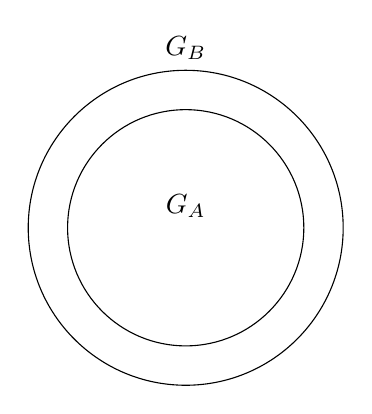
\begin{tikzpicture}[]
            \def\firstcircle{(-1.2,0) coordinate (a) circle (2cm)}
            \def\secondcircle{(-1.2,0) coordinate (b)  circle (1.5cm)}
                \begin{scope}
            \clip \secondcircle;
                \end{scope}
            \draw \firstcircle node[text=black,above] {$G_{A}$};
            \draw \secondcircle;
            \node (c) [above] at (current bounding box.north -| b) {$G_{B}$};
            % \node at (c -| b) {$G_{B}$};
        \end{tikzpicture}
        \caption{Case 1: $G_{A} \subseteq G_{B}$}
        \label{fig:case 1 ga gb}
    \end{subfigure}
    \begin{subfigure}{.5\textwidth}
        \centering
        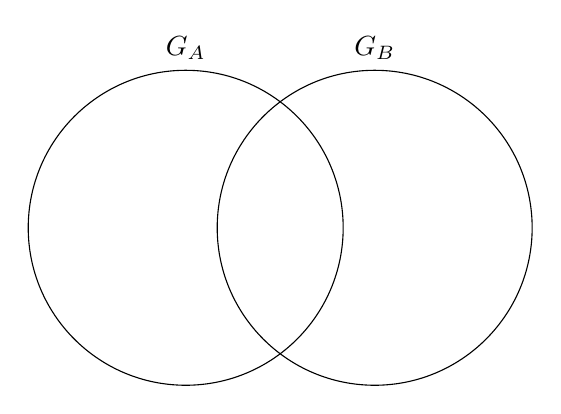
\begin{tikzpicture}[]
            \def\firstcircle{(-1.2,0) coordinate (a) circle (2cm)}
            \def\secondcircle{(1.2,0) coordinate (b)  circle (2cm)}
                \begin{scope}
            \clip \secondcircle;
                \end{scope}
            \draw \firstcircle;
            \draw \secondcircle;
            \node (c) [above] at (current bounding box.north -| a) {$G_{A}$};
            \node at (c -| b) {$G_{B}$};
        \end{tikzpicture}
        \caption{Case 2: $G_{A} \not \subseteq G_{B}$; $G_{A} \cap G_{B} \neq \phi$}
        \label{fig:case 2 ga gb}
    \end{subfigure}
    \newline
    \begin{subfigure}{\textwidth}
        \centering
        \begin{tikzpicture}[]
            \def\firstcircle{(-3,0) coordinate (a) circle (2cm)}
            \def\secondcircle{(3,0) coordinate (b)  circle (2cm)}
                \begin{scope}
            \clip \secondcircle;
                \end{scope}
            \draw \firstcircle;
            \draw \secondcircle;
            \node (c) [above] at (current bounding box.north -| a) {$G_{A}$};
            \node at (c -| b) {$G_{B}$};
        \end{tikzpicture}
        \caption{Case 3: $G_{A} \not \subseteq G_{B}$; $G_{A} \cap G_{B} = \phi$}
        \label{fig:case 3 ga gb}
    \end{subfigure}
    \caption{Interaction of Genres in Treebanks $A$ and $B$, such that $\vert G_{A} \vert \leq \vert G_{B} \vert$}
    \label{fig:GA and GB interactions}
\end{figure}

To see how the $\theta_{pos}$ scores are affected in either of the cases, we perform the following experiment on UDv2.5 \texttt{pl}-LFG data.

\begin{enumerate}
    \item Downsample the number of sentences in \textit{fiction} and \textit{news} genres to 2000 sentences each. Using 2-fold cross-validation, split the downsampled into 2 halves. We refer to one half as \textit{base} set for the genre, and the other as the \textit{test} set for the genre, each containing 1000 sentences.
    \item Downsample the number of sentences in \textit{spoken} genre to 1000 sentences.
    \item Concatenate the downsampled \textit{spoken} data and the \textit{test} set from the other genres. Refer to this dataset as \textit{all\_genres}.
        \begin{equation*}
            \textit{all\_genres} = \textit{spoken} + \textit{fiction\_test} + \textit{news\_test}
        \end{equation*}
    \item Combine the \textit{test} sets to result in \textit{news\_fiction\_test} set.
        \begin{equation*}
            \textit{news\_fiction\_test} = \textit{news\_test} + \textit{fiction\_test}
        \end{equation*}
    \item Combine the \textit{base} sets to result in \textit{news\_fiction\_base} set.
        \begin{equation*}
            \textit{news\_fiction\_base} = \textit{news\_base} + \textit{fiction\_base}
        \end{equation*}
    \item Combine the downsampled \textit{spoken} data with either \textit{test} set to result in \textit{spoken\_genre\_test} data, where \textit{genre} is a placeholder for either of \textit{fiction} or \textit{news}.
        \begin{align*}
            \textit{spoken\_news\_test} & = \textit{spoken} + \textit{news\_test}\\
            \textit{spoken\_fiction\_test} &= \textit{spoken} + \textit{fiction\_test}
        \end{align*}
    \item For Case 1, we study the change in $\theta_{pos}$ score when the data as mentioned in Table \ref{tab:case1_genre} are compared against each other.
        \begin{table}[H]
            \centering
            \begin{tabular}{|c|c|}
                \hline
                \textbf{$G_{A}$} & \textbf{$G_{B}$} \\
                \hline
                $G_{news\_base} = \{news\}$ & $G_{news\_fiction\_test} = \{news, fiction\}$\\
                $G_{news\_base} = \{news\}$ & $G_{spoken\_news\_test} = \{spoken, news\}$\\
                $G_{news\_base} = \{news\}$ & $G_{all\_genres} = \{news, fiction, spoken\}$\\
                \hline
                $G_{fiction\_base} = \{fiction\}$ & $G_{news\_fiction\_test} = \{news, fiction\}$\\
                $G_{fiction\_base} = \{fiction\}$ & $G_{spoken\_fiction\_test} = \{spoken, fiction\}$\\
                $G_{fiction\_base} = \{fiction\}$ & $G_{all\_genres} = \{news, fiction, spoken\}$\\
                \hline
                $G_{news\_fiction\_base} = \{news, fiction\}$ & $G_{all\_genres} = \{news, fiction, spoken\}$\\
                \hline
            \end{tabular}
            \caption{Datasets Compared when $G_{A} \subset G_{B}$ and $\vert G_{A} \vert < \vert G_{B} \vert$}
            \label{tab:case1_genre}
        \end{table}
    \item For Case 2, we study the change in $\theta_{pos}$ score when the data as mentioned in Table \ref{tab:case2_genre} are compared against each other.
        \begin{table}[H]
            \centering
            \begin{tabular}{|c|c|}
                \hline
                \textbf{$G_{A}$} & \textbf{$G_{B}$} \\
                \hline
                $G_{news\_fiction\_base} = \{news, fiction\}$ & $G_{spoken\_news\_test} = \{spoken, news\}$\\
                $G_{news\_fiction\_base} = \{news, fiction\}$ & $G_{spoken\_fiction\_test} = \{spoken, fiction\}$\\
                \hline
            \end{tabular}
            \caption{Datasets Compared when $G_{A} \not \subseteq G_{B}$; $G_{A} \cap G_{B} \neq \phi$ and $\vert G_{A} \vert \leq \vert G_{B} \vert$}
            \label{tab:case2_genre}
        \end{table}
    \item For Case 3, we study the combinations as listed in Table \ref{tab:case3_genre}.
        \begin{table}[H]
            \centering
            \begin{tabular}{|c|c|}
                \hline
                \textbf{$G_{A}$} & \textbf{$G_{B}$} \\
                \hline
                $G_{news\_base} = \{news\}$ & $G_{spoken\_fiction\_test} = \{spoken, fiction\}$\\
                $G_{fiction\_base} = \{fiction\}$ & $G_{spoken\_news\_test} = \{spoken, news\}$\\
                $G_{spoken} = \{spoken\}$ & $G_{news\_fiction\_test} = \{news, fiction\}$\\
                \hline
            \end{tabular}
            \caption{Datasets Compared when $G_{A} \not \subseteq G_{B}$; $G_{A} \cap G_{B} = \phi$ and $\vert G_{A} \vert \leq \vert G_{B} \vert$}
            \label{tab:case3_genre}
        \end{table}
    \item We also calculate $\theta_{pos}$ scores for each \textit{base} and \textit{test} sets with each other, and with \textit{spoken} data, to better know how the scores are being impacted.
    \item We repeat all the above steps 100 times, each with a different seed value to result in differently downsampled data. We present the calculated scores averaged over 100 runs for different cases in Tables \ref{tab:case1_genre-results} - \ref{tab:case3_genre-results}. In the tables, the `Average' column contains the average of means from the preceding columns.
\end{enumerate}

\begin{table}[H]
    \centering
    \begin{tabular}{|c|c|c|c|c|}
        \hline
         & \textit{news\_test} & \textit{fiction\_test} & Average & \textit{news\_fiction\_test}\\
        \hline
        \textit{news\_base} & 0.257 ± 0.01 & 0.646 ± 0.034 & 0.452 & 0.304 ± 0.016 \\
        \textit{fiction\_base} & 0.64 ± 0.034 & 0.278 ± 0.013 & 0.46 & 0.348 ± 0.019 \\
        \hline
    \end{tabular}%
    \vspace{5mm}
    \begin{tabular}{|c|c|c|c|c|}
        \hline
         & \textit{news\_test} & \textit{spoken} & Average & \textit{spoken\_news\_test}\\
        \hline
        \textit{news\_base} & 0.257 ± 0.01 & 1.503 ± 0.049 & 0.88 & 0.489 ± 0.022\\
        \hline
    \end{tabular}%
    \vspace{5mm}
    \begin{tabular}{|c|c|c|c|c|}
        \hline
         & \textit{fiction\_test} & \textit{spoken} & Average & \textit{spoken\_fiction\_test}\\
        \hline
        \textit{fiction\_base} & 0.278 ± 0.013 & 0.99 ± 0.036 & 0.63 & 0.41 ± 0.018\\
        \hline
    \end{tabular}%
    \vspace{5mm}
    \scalebox{0.8}{\begin{tabular}{|c|c|c|c|c|c|}
        \hline
         & \textit{news\_test} & \textit{fiction\_test} & \textit{spoken} & Average & \textit{all\_genres}\\
        \hline
        \textit{news\_base} & 0.257 ± 0.01 & 0.646 ± 0.034 & 1.503 ± 0.049 & 0.802 & 0.463 ± 0.022\\
        \textit{fiction\_base} & 0.64 ± 0.034 & 0.278 ± 0.013 & 0.99 ± 0.036 & 0.64 & 0.351 ± 0.014\\
        \textit{news\_fiction\_base} & 0.3 ± 0.015 & 0.351 ± 0.021 & 1.144 ± 0.035 & 0.6 & 0.247 ± 0.011\\
        \hline
    \end{tabular}}
    \caption{Case 1}
    \label{tab:case1_genre-results}
\end{table}

\begin{table}[H]
    \centering
    \scalebox{0.9}{\begin{tabular}{|c|c|c|c|c|}
        \hline
         & \textit{spoken} & \textit{news\_test} & Average & \textit{spoken\_news\_test}\\
        \hline
        \textit{news\_base} & 1.503 ± 0.049 & 0.257 ± 0.01 & 0.88 & 0.489 ± 0.022\\
        \textit{fiction\_base} & 0.99 ± 0.036 & 0.64 ± 0.034 & 0.81 & 0.499 ± 0.02\\
        \textit{news\_fiction\_base} & 1.144 ± 0.035 & 0.3 ± 0.015 & 0.7 & 0.498 ± 0.023\\
        \hline
    \end{tabular}}%
    \vspace{5mm}
    \scalebox{0.9}{\begin{tabular}{|c|c|c|c|c|}
        \hline
         & \textit{spoken} & \textit{fiction\_test} & Average & \textit{spoken\_fiction\_test}\\
        \hline
        \textit{news\_base} & 1.503 ± 0.049 & 0.646 ± 0.034 & 1.075 & 0.854 ± 0.036\\
        \textit{fiction\_base} & 0.99 ± 0.036 & 0.278 ± 0.013 & 0.63 & 0.41 ± 0.018\\
        \textit{news\_fiction\_base} & 1.144 ± 0.035 & 0.351 ± 0.021 & 0.747 & 0.498 ± 0.023\\
        \hline
    \end{tabular}}
    \caption{Case 2}
    \label{tab:case2_genre-results}
\end{table}

\begin{table}[H]
    \centering
    \begin{tabular}{|c|c|c|c|c|}
        \hline
         & \textit{spoken} & \textit{fiction\_test} & Average & \textit{spoken\_fiction\_test}\\
        \hline
        \textit{news\_base} & 1.503 ± 0.049 & 0.646 ± 0.034 & 1.075 & 0.854 ± 0.036\\
        \hline
    \end{tabular}%
    \vspace{5mm}
    \begin{tabular}{|c|c|c|c|c|}
        \hline
         & \textit{spoken} & \textit{news\_test} & Average & \textit{spoken\_news\_test}\\
        \hline
        \textit{fiction\_base} & 0.99 ± 0.036 & 0.64 ± 0.034 & 0.81 & 0.499 ± 0.02\\
        \hline
    \end{tabular}%
    \vspace{5mm}
    \begin{tabular}{|c|c|c|c|c|}
        \hline
         & \textit{news\_test} & \textit{fiction\_test} & Average & \textit{news\_fiction\_test}\\
        \hline
        \textit{spoken} & 1.493 ± 0.048 & 0.987 ± 0.034 & 1.24 & 1.138 ± 0.03\\
        \hline
    \end{tabular}
    \caption{Case 3}
    \label{tab:case3_genre-results}
\end{table}

From the tables, it can be observed that the decomposition of a treebank into its constituent genres forms the first basis for the combination of the different genres. Once the individual genres have been identified and checked for the inter-generic $\theta_{pos}$ scores, the overall metric score is less than the average of the metric scores calculated for individual pair of genres in the treebank(s). Upon a closer inspection, it was discovered that when there are multiple genres present in the treebank, the $\theta_{pos}$ metric score is dominated by the POS trigrams that are typical of the language, and the genre-specific POS trigrams become more and more obscure.

Assuming treebanks $A$ and $B$ can be split into their constituent genres such that $G_{A} = \{A_{1}, A_{2}, ... , A_{i}\}$ and $G_{B} = \{B_{1}, B_{2}, ... , B_{j}\}$, the overall limit on the $\theta_{pos}(A, B)$ score can be specified as in Equation \ref{eqn:theta_pos_combo_limit}.

\begin{equation}
    \boxed{\theta_{pos}(A, B) \leq \Theta_{pos}(A, B) = Average(\theta_{pos}(A_{x}, B_{y}))} \hspace{5mm} \forall [A_{x} \in G_{A}; B_{y} \in G_{B}]
\label{eqn:theta_pos_combo_limit}
\end{equation}

\section{Framing Overall \texorpdfstring{$\Theta_{pos}$}{Theta\_pos} Limit}
\label{sec:pos-harmony-calculations}

We studied the effects of size and genre variation in treebanks in the previous sections. It was stated earlier that in order for two datasets to be compared, they should satisfy the condition as mentioned in Equation \ref{eqn:size_constraint} (restated below).

\begin{equation}
\boxed{size(A) \geq 400 \And Avg(A) \geq Avg(B) \implies size(B) \cdot \frac{Avg(B)}{Avg(A)} \geq 400} \tag{\ref{eqn:size_constraint}}
\end{equation}

 where

\begin{enumerate}
    \item $Avg(X) = \frac{Total Syntactic Words(X)}{size(X)}$ is the average sentence length in dataset $X$
    \item $size(X)$ refers to the number of sentences in dataset $X$
\end{enumerate}

For given datasets of the same genre such that the datasets satisfy the condition in Equation \ref{eqn:size_constraint} above, the upper limit on the $\theta_{pos}$ metric score for the datasets to be deemed as consistent in their annotation is specified in Equation \ref{eqn:theta_pos_size_limit} (restated below).

\begin{equation}
\boxed{\theta_{pos}(A,B) \leq \Theta_{pos}(A,B) = 0.5}  \tag{\ref{eqn:theta_pos_size_limit}}
\end{equation}

The different genres possible in a treebank can be analysed in two aspects. The first aspect looks at the formality and informality level within a genre, given by the genre's F-measure and I-measure respectively. While the original terms were defined on the basis of the frequency of the different POS tags, we worked with normalised frequency counts of the different POS tags to make the measures comparable against different treebanks, irrespective of their size. 

\textbf{Add stuff here}

For the different treebanks that are present in two treebanks, the limit on the $\theta_{pos}$ metric can be determined by the average score of the $\theta_{pos}$ scores calculated by Equation ref{eqn:theta-limit-genre} between different genres present in the treebanks, such that the dataset from the genres satisfy the equation \ref{eqn:theta_pos_combo_limit}.
% There are a large number of genres that are not covered in our approach. However, we can come up with a theoretical limit nonetheless. We can describe our coverage of genres in 3 broad categories, viz. print media (\textit{fiction}, \textit{news}, \textit{nonfiction}), social media (\textit{blog}, \textit{social}) and spoken data (\textit{spoken}). There exists an overlap between the categories. However, any genre that is not included can almost always be classified within the realm of the categories defined above. It is important to note that the categories should be considered as points in the continuous range, and not as discreet ones in themselves. From there, we can establish the upper limits on the variability of \(\theta_{POS}\) score as in Table \ref{tab:thetapos_genre}.

% \begin{table}[h]
%     \centering
%     \begin{tabular}{|c|c|c|}
%     \hline
%     \textbf{Category 1} & \textbf{Category 2} & \textbf{Limit} \\
%     \hline
%     Print & Social & 0.8 \\
%     Print & Spoken & 1.4 \\
%     Social & Spoken & 1.4 \\
%     \hline
%     \end{tabular}
%     \caption{Limits on \(\theta_{POS}\) for Genre-based Disparity}
%     \label{tab:thetapos_genre}
% \end{table}

% \section{Discussion and Conclusion}
% \label{sec:pos-harmony-conclusion}

% \subsection{Unaccounted Factors}
% \subsubsection{Out of Vocabulary Words}

% The metric \(\theta_{pos}\) uses POS trigrams to compute the divergence of the annotation. Since the metric is delexicalised, the concept of out-of-vocabulary (OOV) words does not make sense in the calculation of the metric score. In case of either treebank being annotated (semi-)automatically by a POS tagger, the improper annotation of OOV words can affect the scores negatively.

% In UD tagset, \verb|X| tag is reserved for words such that they can not be categorised under any of the other POS. While it is recommended to be used in a restricted manner\footnote{\url{https://universaldependencies.org/u/pos/X.html}}, the tag can exhibit itself abundantly depending on the origin source of the data, with the genres containing Web2.0 data being especially susceptible.

% For most treebanks, the influence of OOV words should be minimal. Nonetheless, care must be taken when the \verb|X| tag is present in the trigrams of either of the treebanks.

% \subsection{Conclusion}

% In practice, it is not always possible to get an estimate of the annotation quality of individual treebanks. Neither of the aforementioned assumptions can be made in such cases. If either of the treebanks in a considered pair can be estimated for quality, the other treebank can be compared for a similar annotation quality. However, like in the x 
% \textbf{ELABORATE}
% \textbf{blah}